% fig6_ablation — ablation attribution (beneficial effect)
% 用途: 交底书 图6, §六: random 20 点消融, 相对总等效电量距离 (full=100)
% 数据: results/table_20260819_105511.md 消融 random_20p 组 (cost mean):
%   full 100.0 / nn_only 105.2 / no_oropt 103.1 / no_2opt 100.2 / fixed_payload 114.6
%   (fixed_payload = 忽略载重耦合: 构造+搜索用 beta=0, 真实 beta 评估)
% 编译: latexmk -pdf -xelatex fig6_ablation.tex
\documentclass[tikz,border=8pt]{standalone}
\usepackage{amsmath}
\usepackage{pgfplots}
\pgfplotsset{compat=1.18}
\begin{document}
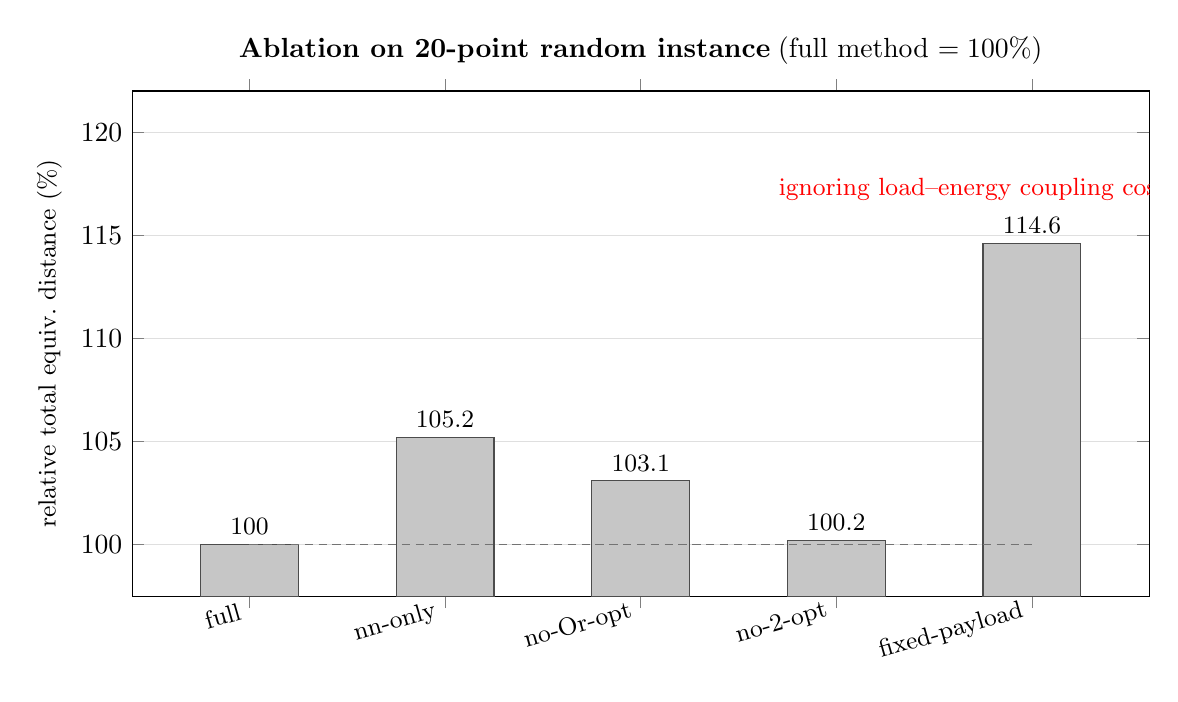
\begin{tikzpicture}
\begin{axis}[
  width=14.5cm, height=8cm,
  ybar, bar width=0.5,
  xmin=0.4, xmax=5.6,
  xtick={1,2,3,4,5},
  xticklabels={full, nn-only, no-Or-opt, no-2-opt, fixed-payload},
  x tick label style={rotate=16, anchor=east, font=\small},
  ylabel={relative total equiv.\ distance (\%)},
  ymin=97.5, ymax=122,
  ymajorgrids, grid style={gray!25},
  nodes near coords, every node near coord/.append style={font=\small, anchor=south},
  title={\textbf{Ablation on 20-point random instance}\;(full method $=100\%$)},
  label style={font=\small},
]
\addplot[draw=black!70, fill=gray!45] coordinates {
  (1,100) (2,105.2) (3,103.1) (4,100.2) (5,114.6)};
% baseline at full=100 (numeric x works inside ybar axis)
\draw[densely dashed, black!55] (axis cs:1,100) -- (axis cs:5,100);
\node[red,font=\small,anchor=south,align=center] at (axis cs:5,116.2)
  {ignoring load--energy coupling costs {\bf +14.6\%}};
\end{axis}
\end{tikzpicture}
\end{document}
